\documentclass[17pt,mathserif]{beamer}
\usetheme{Singapore}
\usecolortheme{orchid}
\AtBeginSection{\frame{\sectionpage}}

\usepackage[english]{babel}
\usepackage[english]{isodate}
\cleanlookdateon

\usepackage{amsmath}
\usepackage{listings}
\usepackage[thicklines]{cancel}
\usepackage{pgfgantt}
\usepackage{array}
\usepackage{calc}

\newcommand{\oclass}[1]{\ensuremath{\mathtt{#1}}}
\newcommand{\osub}{\sqsubseteq}

\begin{document}

\title{Ontology Unit Testing}
\subtitle{Towards Test-Driven Development}
\author{Ameerah Allie \and Kieren Davies}
\institute[UCT]{University of Cape Town}
\date{\printdate{2016-05-25}}
\titlepage

\begin{frame}
  \frametitle{Outline}
  \tableofcontents
\end{frame}

\section{Context}

\begin{frame}{Ontology engineering}
  \begin{itemize}
    \item Formal representation of knowledge
    \item Automated reasoning
  \end{itemize}
  \centering
  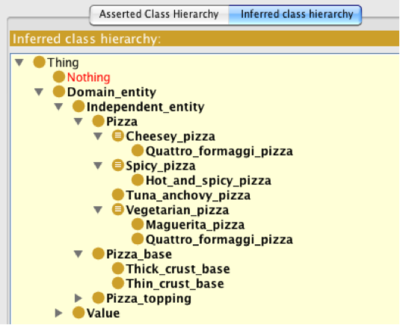
\includegraphics[width=0.5\textwidth]{pizza}
\end{frame}

\begin{frame}{Test-driven development}
  \begin{itemize}
    \item Successful in software engineering
    \item Ontology engineering less mature
    \begin{itemize}
      \item Test-last
      \item ``Try-and-see'' with reasoner
      \item First test harnesses in 2015
    \end{itemize}
  \end{itemize}
\end{frame}
\note{
  TDD:
  \begin{itemize}
    \item understandability
    \item reduced complexity
    \item code quality
    \item reliability: external tests passed
  \end{itemize}
}

\begin{frame}{Why test?}
  \begin{align*}
    \oclass{Giraffe} &\osub \oclass{Herbivore} \\
    \oclass{Herbivore} &\osub \oclass{Mammal} \phantom{\; \oclass{Animal}} \\
    \oclass{Mammal} &\osub \oclass{Animal}
  \end{align*}
  \[ \mathrm{mammals} = \{\dots, \oclass{Giraffe} ,\dots\} \]
\end{frame}

\begin{frame}{Why test?}
  \begin{align*}
    \oclass{Giraffe} &\osub \oclass{Herbivore} \\
    \oclass{Herbivore} &\osub \cancel{\oclass{Mammal}} \; \oclass{Animal} \\
    \oclass{Mammal} &\osub \oclass{Animal}
  \end{align*}
  \[ \mathrm{mammals} = \{\dots, \cancel{\oclass{Giraffe}} ,\dots\} \]
\end{frame}
\note{
  Listing mammals misses giraffe
}

\begin{frame}{Related work}
  \begin{itemize}
    \item Vrande\v{c}i\'c and Gangemi
    \item Tawny-OWL (Warrender and Lord)
    \item SCONE (Neuhaus)
    \item TDDOnto ({\L}awrynowicz and Keet)
    \item OWL Reasoner Evaluation competition
  \end{itemize}
\end{frame}

\begin{frame}{Vrande\v{c}i\'c and Gangemi}
  \begin{align*}
    O &\models A_i^{+} \quad \forall A_i^{+} \in T^{+} \\
    O &\not\models A_i^{-} \quad \forall A_i^{-} \in T^{-}
  \end{align*}
\end{frame}
\note{
  No implementation
}

\begin{frame}[fragile]{Tawny-OWL}
  \begin{lstlisting}[language=Lisp,basicstyle=\normalsize\ttfamily]
(is
  (r/superclass?
    i/k46_XY
    n/MaleKaryotype))
  \end{lstlisting}
\end{frame}

\begin{frame}[fragile]{SCONE}
  \begin{lstlisting}[basicstyle=\footnotesize\ttfamily]
Scenario: Relative age between family members
  The parenthood relation entail an ordering of age.
  Given Chris is a parent of Dora.
  And Amy is a parent of Chris.
  And Amy is a parent of Berta.
  Then infer Chris is older than Dora.
  And infer Amy is older than Dora.
  And don’t infer Berta is older than Dora.
  And don’t infer Dora is older than Dora.
  \end{lstlisting}
\end{frame}

\begin{frame}{TDDOnto}
  \begin{itemize}
    \item Prot\'eg\'e plugin
  \end{itemize}
  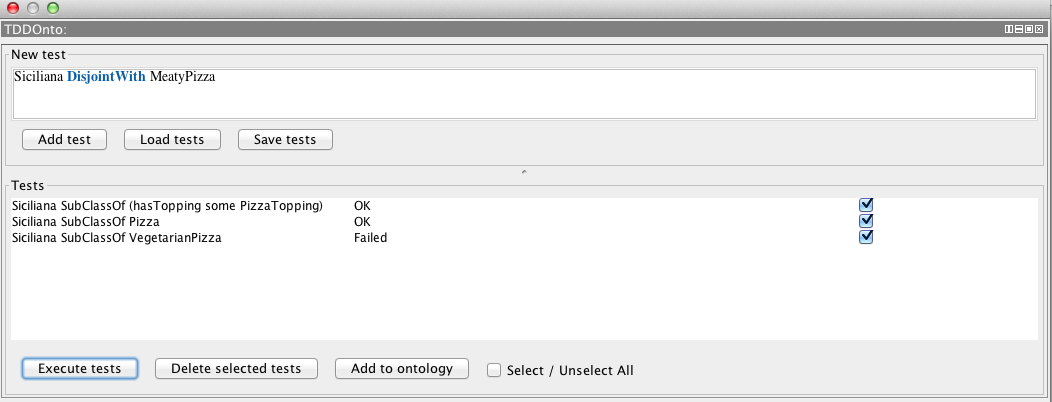
\includegraphics[width=\textwidth]{tddonto}
\end{frame}

\begin{frame}{OWL Reasoner Evaluation}
  \begin{itemize}
    \item Comparison of reasoner performance
    \item 14 reasoners tested
    \item Only OWL 2 DL and EL
  \end{itemize}
\end{frame}

\section{Problem}

\begin{frame}{Problem}
  \begin{itemize}
    \item Available tools don't support comprehensive tests
    \begin{itemize}
      \item No systematic coverage of OWL features
      \item e.g.\ ABox assertions, RBox
    \end{itemize}
    \item Not formally verified
    \begin{itemize}
      \item Only empirically
    \end{itemize}
    \item Performance of reasoner-based tests poorly understood
  \end{itemize}
\end{frame}

\begin{frame}{Task: New tests}
  \begin{itemize}
    \item Describe and implement new unit tests
    \begin{itemize}
      \item Systematically address OWL features
      \item Complex axioms
    \end{itemize}
    \item Prove correctness of algorithms
  \end{itemize}
\end{frame}

\begin{frame}{Research question: Benchmarking}
  \centering
  Which reasoner performs best on each of the unit test implementations in real ontologies?
\end{frame}

\begin{frame}{Aims}
  \begin{itemize}
    \item Improve ontology engineering process by
    \begin{itemize}
      \item defining and implementing more tests
      \item proving their correctness
      \item determining test performance of reasoners
    \end{itemize}
  \end{itemize}
\end{frame}

\begin{frame}{Benefits}
  \begin{itemize}
    \item Improve ontology quality, reduce complexity, improve understandability
    \item Encourage wider adoption of ontologies
  \end{itemize}
\end{frame}

\section{Methods}

\begin{frame}{New tests}
  \begin{enumerate}
    \item Create formal model
    \item Prove correctness of a test implemented in TDDOnto
    \item Describe new tests
    \item Prove correctness
    \item Implement
  \end{enumerate}
\end{frame}

\begin{frame}[allowframebreaks]{Benchmarking}
  \begin{enumerate}
    \item Gather ontologies
    \item Implement/obtain algorithm to generate unit tests
    \item Implement/obtain benchmark wrapper script
    \item Benchmarking one test type in one ontology
    \item Identify independent variables
    \item Modify script to do every combination of chosen variables
    \item Perform benchmarks, record results
    \item Statistical tests on resulting data
  \end{enumerate}
\end{frame}
\note{
  \begin{itemize}
    \item First benchmark to check script and test generation
    \item Independent variables e.g.\ DL profile, ontology size
  \end{itemize}
}

\section{Outcomes}

\begin{frame}{Expected outcomes}
  \begin{itemize}
    \item Create suite of tests
    \begin{itemize}
      \item Approaching comprehensiveness
      \item Proven correct
    \end{itemize}
    \item Benchmark reasoners
    \begin{itemize}
      \item Statistically significant differences
      \item Better understand reasoner performance
      \item Inform choice of reasoners for future work
    \end{itemize}
  \end{itemize}
\end{frame}
\note{
  If not significant, still fine
}

\section{Plan}

\begin{frame}{Division of work}
  \begin{itemize}
    \item Kieren: new tests
    \item Ameerah: benchmarking
  \end{itemize}
\end{frame}

\begin{frame}{Timeline}
  \resizebox{\textwidth}{!}{\begin{ganttchart}[
  time slot format = isodate,
  calendar week text = \currentweek,
  title height = 1,
  y unit title = 0.5cm,
  y unit chart = 0.45cm,
  x unit = 0.1cm,
  vgrid = {*6{gray!10}, {gray!40}},
  hgrid = gray!40,
  group peaks width = 1.5,
  group left shift = -0.5,
  group right shift = 0.5,
  bar/.append style = {fill=gray!20},
  ]{2016-05-02}{2016-11-20}
  \gantttitle{Block 2}{40} \gantttitle{Vacation}{37} \gantttitle{Block 3}{40} \gantttitle{Block 4}{86} \\
  \gantttitlecalendar{month=name, week} \\

  \ganttgroup{Proposal}{2016-05-04}{2016-06-10} \\
  \ganttbar{Proposal}{2016-05-04}{2016-05-17} \\
  \ganttbar{Proposal presentation}{2016-05-18}{2016-05-25} \\
  \ganttbar{Revised proposal}{2016-05-18}{2016-06-08} \\
  \ganttbar{Website}{2016-05-26}{2016-06-10} \\[hgrid style/.style=solid]

  \ganttgroup{New test/proof feasibility}{2016-06-11}{2016-07-17} \\
  \ganttbar{Formal model}{2016-06-11}{2016-06-19} \\
  \ganttbar{Prove an existing test}{2016-06-20}{2016-06-23} \\
  \ganttbar{Describe/prove new tests}{2016-06-24}{2016-07-10} \\
  \ganttbar{Implement one test}{2016-07-11}{2016-07-17} \\

  \ganttgroup{Benchmarking feasibility}{2016-06-11}{2016-07-17} \\
  \ganttbar{Gather ontologies and scripts}{2016-06-11}{2016-06-13} \\
  \ganttbar{Adapt benchmark scripts}{2016-06-14}{2016-06-26} \\
  \ganttbar{Experiment with parameters}{2016-06-27}{2016-07-03} \\
  \ganttbar{Run subset of benchmarks}{2016-07-04}{2016-07-05} \\
  \ganttbar{Analyse data}{2016-07-06}{2016-07-17} \\[hgrid style/.style=solid]

  \ganttgroup{Further development}{2016-07-23}{2016-09-19} \\
  \ganttbar{Prove/implement further tests}{2016-07-23}{2016-09-19} \\
  \ganttbar{Extend benchmarks}{2016-07-23}{2016-09-19} \\
  \ganttbar{Benchmark new tests}{2016-08-22}{2016-09-19} \\[hgrid style/.style=solid]

  \ganttgroup{Paper write-up}{2016-07-11}{2016-10-27} \\
  \ganttbar{Background}{2016-07-11}{2016-07-21} \\
  \ganttbar{Plan with revisions}{2016-07-22}{2016-08-28} \\
  \ganttbar{First experiment}{2016-09-06}{2016-09-19} \\
  \ganttbar{Final experiment}{2016-09-20}{2016-09-28} \\
  \ganttbar{Implementation and testing}{2016-09-29}{2016-10-03} \\
  \ganttbar{Complete outline}{2016-10-04}{2016-10-10} \\
  \ganttbar{Remaining sections}{2016-10-11}{2016-10-17} \\
  \ganttbar{Final changes}{2016-10-18}{2016-10-27} \\[hgrid style/.style=solid]

  \ganttbar{Demonstration}{2016-10-28}{2016-10-31} \\
  \ganttbar{Poster}{2016-11-01}{2016-11-06} \\
  \ganttbar{Website}{2016-11-07}{2016-11-10} \\
  \ganttbar{Reflection paper}{2016-11-11}{2016-11-13}
\end{ganttchart}
}
\end{frame}

\begin{frame}{Risks}
  \hyphenpenalty=10000
  \footnotesize
  \renewcommand{\arraystretch}{2}
  \begin{tabular}{@{}>{\raggedright}p{0.5\textwidth-\tabcolsep}>{\raggedright\arraybackslash}p{0.5\textwidth-\tabcolsep}@{}}
    BM on desktop too slow &
    UCT grid cluster, parallelise \\ \hline
    Formal model too difficult &
    Get help from DL experts \\ \hline
    BM scripts not available &
    Write from scratch, reduce scope \\ \hline
    BM scripts can't be adapted &
    Help from Dr.\ {\L}awrynowicz, rewrite scripts, reduce scope \\ \hline
    Can't implement tests in {TDDOnto} &
    Use another tool, develop new tool
  \end{tabular}
\end{frame}

\begin{frame}{Ethical, legal, professional}
  \begin{itemize}
    \item Software licensing
    \begin{itemize}
      \item Prot\'eg\'e, TDDOnto, reasoners, scripts
      \item Our implementations
      \item Gathered ontologies
    \end{itemize}
    \item UCT IP policies
  \end{itemize}
\end{frame}

\end{document}
